\documentclass[czech, kiv, ba, he, iso690numb, pdf, viewonly]{fasthesis}

\usepackage{url}
\usepackage{enumitem}
\usepackage{forest}
\usepackage{tikz}

\definecolor{folderbg}{RGB}{124,166,198}
\definecolor{folderborder}{RGB}{110,144,169}

\lstdefinelanguage{json}{
    basicstyle=\ttfamily\small,
    showstringspaces=false,
    backgroundcolor=\color{white},
    literate=
     *{0}{{{\color{blue}0}}}{1}
      {1}{{{\color{blue}1}}}{1}
      {2}{{{\color{blue}2}}}{1}
      {3}{{{\color{blue}3}}}{1}
      {4}{{{\color{blue}4}}}{1}
      {5}{{{\color{blue}5}}}{1}
      {6}{{{\color{blue}6}}}{1}
      {7}{{{\color{blue}7}}}{1}
      {8}{{{\color{blue}8}}}{1}
      {9}{{{\color{blue}9}}}{1}
      {:}{{{\color{red}:}}}{1}
      {,}{{{\color{red},}}}{1}
      {\{}{{{\color{black}\{}}}{1}
      {\}}{{{\color{black}\}}}}{1}
      {[}{{{\color{black}[}}}{1}
      {]}{{{\color{black}]}}}{1},
}

\title{Implementace modulu pro import údajů RÚIAN}
\author{Martin}{Schön}{}{}
\supervisor{Ing. Martin Bíkl, Ing. Petr Přibyl, Ing. Martin Zíma Ph.D.}
\stagworkid{100718}
\assignment{figures/A22B0144P_Zadani.pdf}
\signdate{5}{5}{2025}{V Plzni}
\addbibresource{bib.bib}
\abstract{
    Tato bakalářská práce se zabývá návrhem a implementací softwarového modulu pro 
    import údajů z~Registru územní identifikace, adres a nemovitostí (RÚIAN) do 
    relačních databázových systémů. Cílem práce bylo vytvořit konfigurovatelnou aplikaci 
    umožňující stahování, zpracování a synchronizaci údajů z~RÚIAN do databází PostgreSQL, 
    Microsoft~SQL~Server a Oracle. Řešení je postaveno na jazyce Java s~využitím frameworku 
    Spring~Boot, Hibernate~ORM a plánovače Quartz~Scheduler. Součástí práce je návrh konfiguračního 
    souboru ve formátu JSON, podpora přírůstkového i~kompletního stahování dat a optimalizace výkonu 
    při práci s~velkými datovými objemy. Výsledná aplikace byla otestována na reálných datech a ověřena 
    z~hlediska správnosti importu a rychlosti zpracování.
}
{
    This bachelor's thesis focuses on the design and implementation of a software module for 
    importing data from the Czech Register of Territorial Identification, Addresses, and Real 
    Estate (RÚIAN) into relational database systems. The aim was to create a configurable application 
    enabling the download, processing, and synchronization of RÚIAN data into PostgreSQL, 
    Microsoft SQL Server, and Oracle databases. The solution is based on Java, utilizing the 
    Spring Boot framework, Hibernate ORM, and the Quartz Scheduler. The work includes the design of a 
    JSON configuration file, support for both incremental and full data downloads, and performance 
    optimization for large datasets. The resulting application was tested on real data and verified 
    for data import accuracy and processing speed.
}
\keywords{RÚIAN, databáze, import, aplikace, Java, PostgreSQL, Oracle, Microsoft SQL}
\acknowledgement{
    Rád bych poděkoval vedoucím své bakalářské práce, Ing.~Martinu Bíklovi a~Ing.~Martinu Zímovi, Ph.D., za jejich cenné rady, 
    trpělivost a~odborné vedení, které mi poskytovali během celé doby řešení této práce. Dále děkuji své rodině a~blízkým za podporu, 
    motivaci a~trpělivost, bez které by dokončení této práce nebylo možné.
\begin{flushright}
    \textit{Martin Schön} \\
    autor práce \\
    (duben 2025)
\end{flushright}
}
\begin{document}
\frontpages[tm]
\tableofcontents
%1--------------------------------------------------------------------------

\chapter{Úvod}
Problematika správy uzemní identifikace a prostorových dat a~jejich synchronizace mezi různými systémy
nabývá na významu s~rostoucí digitalizací státní správy a~soukromých sektorů.
Jedním z~klíčových zdrojů těchto dat v~České republice je Registr územní identifikace,
adres a~nemovitostí (RÚIAN), který poskytuje rozsáhlé a~aktuální informace o~územních
objektech, adresách a~dalších klíčových entitách. Efektivní využití dat z~RÚIAN vyžaduje
nejen jejich přístup prostřednictvím datových služeb, ale také robustní řešení pro mapování,
konfiguraci a~synchronizaci datových struktur.

Cílem této bakalářské práce je analyzovat datové schéma registru RÚIAN a~možnosti získávání
dat prostřednictvím nabízených datových služeb. Dále bude provedena analýza a~návrh konfiguračního
řešení, které umožní nastavit úroveň přenášených územních objektů a~cílové databázové struktury.
V~rámci práce bude navržena a~implementována aplikace, která umožní pravidelnou synchronizaci dat
z~veřejné databáze RÚIAN do cílových databázových struktur s~podporou databází Oracle,
Microsoft~SQL Server a~PostgreSQL. Aplikace bude schopna provádět synchronizaci kompletních datových
sad i~přírůstkových změn podle zadané konfigurace.

\chapter{RÚIAN}
RÚIAN je zkratkou pro Registr územní identifikace, adres a~nemovitostí.
Jedná se o~státní informační systém v~České republice, který obsahuje informace o~adresách, budovách, parcelách a~dalších objektech.
Systém je spravován Českým úřadem zeměměřickým a~katastrálním (ČÚZK).
Data jsou využívána v~mnoha oblastech, například v~urbanistickém plánování, geodézii nebo při správě nemovitostí.
Jednotlivé prvky jsou zobrazovány na~mapách státního mapového díla a~digitální mapě veřejné správy.

Data z~RÚIAN jsou veřejně dostupná a~lze je získat z~webové služby na~adrese \url{https://vdp.cuzk.gov.cz/vdp/ruian}.
Lze stahovat data ve~formátu XML, která obsahují základní nebo úplné informace o~územních prvcích.
Mezi tyto prvky patří Stát, VÚSC (Vyšší územní samosprávný celek), ORP (Obec s~rozšířenou působností), Obec, Část obce, Ulice, Adresa atd.
Data lze vyhledávat, ověřovat a~stahovat dle jednotlivých územních prvků, které jsou uloženy v~databázi RÚIAN.

\section{Výměnný formát RÚIAN}
Výměnný formát RÚIAN (VFR) je jednou ze služeb, které poskytuje ČÚZK.
Tento formát slouží k~přenosu dat mezi různými informačními systémy.

Je možné stahovat data podle zadaných formátů: \textbf{Standardní}, \textbf{Historický} a~\textbf{Speciální}.
Dále je možné si vybrat mezi přírůstkovými daty a~úplnou kopií.
Přírůstky je možné vyhledávat podle data -- od~zvoleného dne až do~současnosti.
Úplná kopie obsahuje všechna data a~je možné ji také časově vymezit. Tato data se aktualizují jednou měsíčně.

Každý formát navíc nabízí další parametry, které lze nastavit.
Data z~VFR jsou ve~formátu XML.
Každý XML element obsahuje atributy, které nesou informace o~dané entitě (tabulce).

\newpage

\begin{itemize}
    \item \textbf{Standardní} -- obsahuje úplná nebo přírůstková data.
    \begin{itemize}[itemsep=0pt]
        \item Časový rozsah: přírůstky od~data / úplná kopie,
        \item Územní prvky: Stát až~ZSJ / Obec a~podřazené,
        \item Datová sada: základní / kompletní,
        \item Výběr údajů: základní údaje / generované hranice, originální hranice, vlajky a~znaky,
        \item Územní omezení: ČR / kraj (VÚSC) / ORP / obec,
    \end{itemize}

    \item \textbf{Historický} -- obsahuje historická data.
    \begin{itemize}[itemsep=0pt]
        \item Časový rozsah: přírůstky od~data / úplná kopie,
        \item Územní prvky: Stát až~ZJS / Obec a~podřazené,
        \item Územní omezení: ČR / kraj (VÚSC) / ORP / obec,
    \end{itemize}

    \item \textbf{Speciální} -- obsahuje speciální datové sady.
    \begin{itemize}[itemsep=0pt]
        \item Časový rozsah: přírůstky od~data / úplná kopie,
        \item Výběr údajů: číselníky / vazby / vazby a~číselníky,
        \item Kategorie: všechny / geodetické body / nerostné bohatství,
    \end{itemize}
\end{itemize}

\section{Datové struktury}
Data z~RÚIAN jsou rozdělena do~několika datových struktur neboli entit.
Jak je vidět na obrázku~\ref{fig:ruian_tables} \cite{ruian_vfr}, každá entita obsahuje specifické informace.
Mezi tyto informace patří například název státu, kód státu, geografické souřadnice, datum vzniku a~další. 

Stát představuje nejvyšší úroveň hierarchie, pod kterou spadají další entity závislé na~ní.
Příkladem je entita \textbf{VÚSC}, která obsahuje informace o~vyšších územních samosprávných celcích.
Jednotlivé entity na~sebe navzájem odkazují pomocí cizích klíčů.

\begin{figure}[!h]
    \centering
    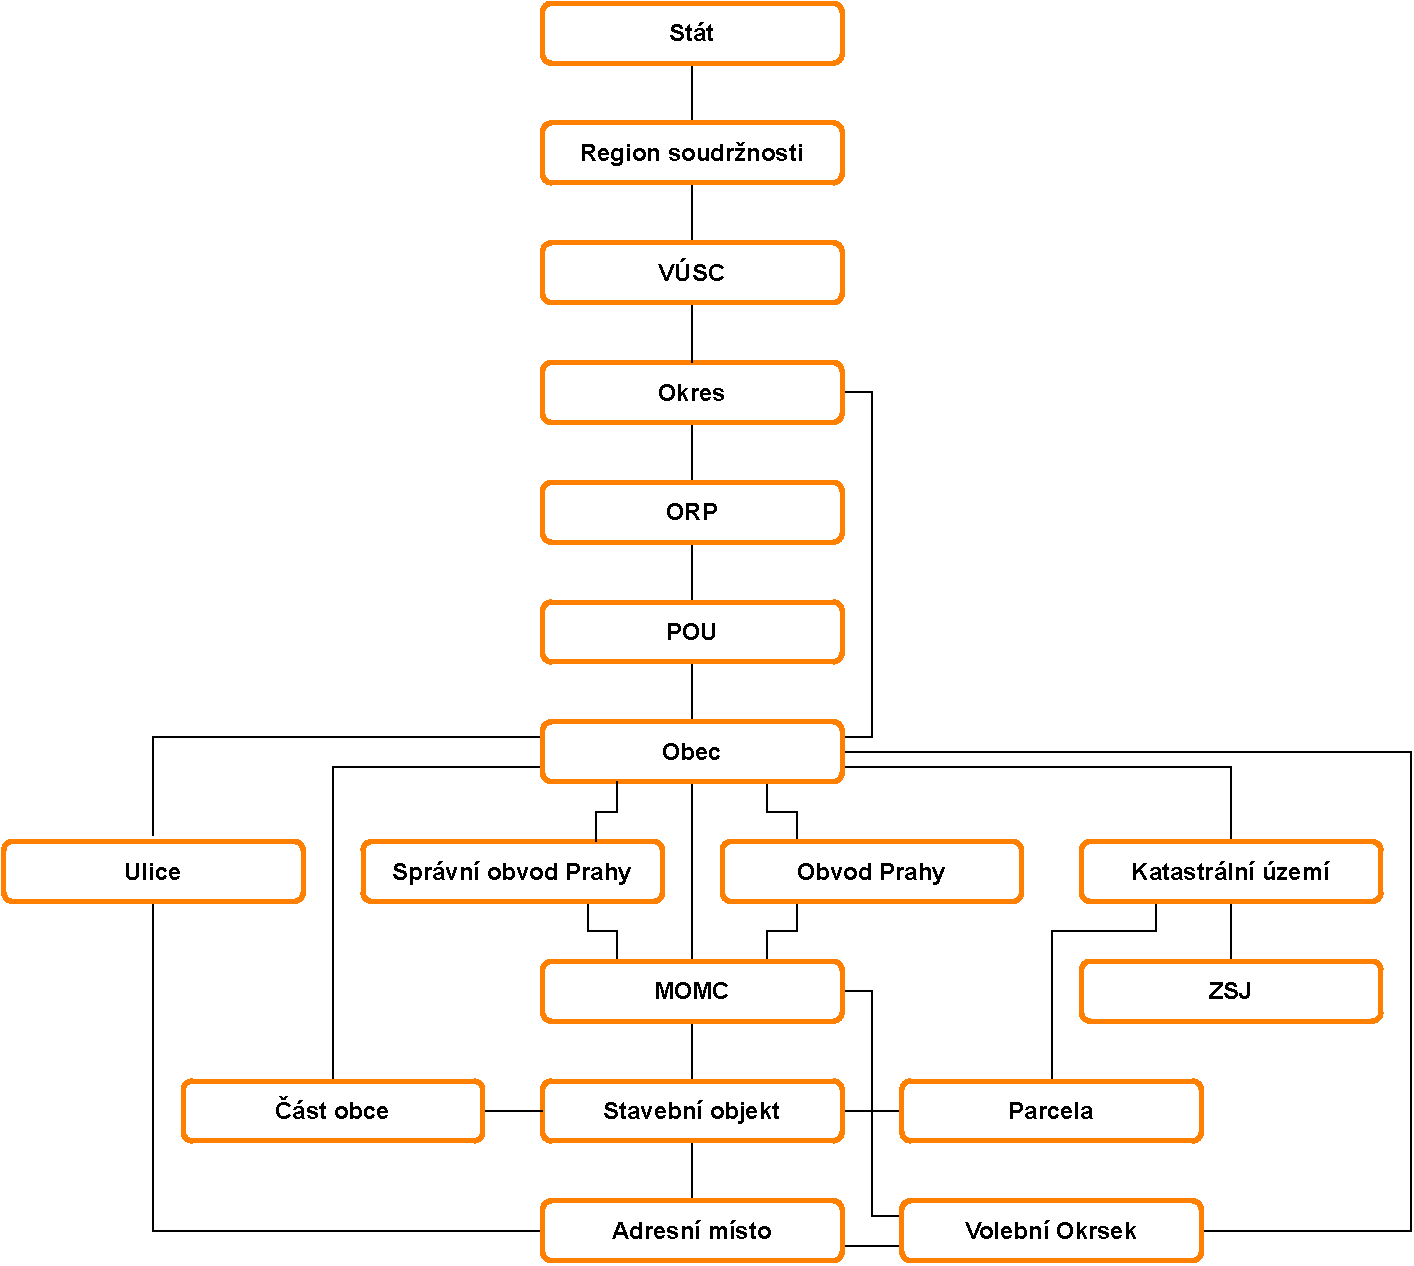
\includegraphics[width=\textwidth]{figures/ruian_diagram.pdf}
    \caption{Schéma prvků RÚIAN}
    \label{fig:ruian_tables}
\end{figure}

\newpage

\section{Formát dat}
Data z~RÚIAN jsou ve~formátu XML. Tento formát je strukturovaný a~umožňuje přenášet data mezi různými systémy.
Bude proto třeba implementovat parser, který převede data z~XML do~dále zpracovávaného formátu pro databáze.


\chapter{Databázové systémy}
Databázový systém je softwarový nástroj, který slouží k~efektivnímu ukládání, organizaci a~vyhledávání dat.
Díky své strukturované povaze umožňuje správu velkých objemů dat a~poskytuje funkcionality pro
zajištění konzistence, bezpečnosti a~rychlého přístupu k~uloženým informacím.

Databázový systém lze obecně rozdělit do~dvou hlavních kategorií: \textbf{relační} a~\textbf{objektový databázový systém}.
Každý z~těchto přístupů má své specifické vlastnosti a~je vhodný pro odlišné typy aplikací.

\subsubsection*{Relační databázové systémy}
\begin{itemize}[itemsep=-1pt]
    \item Data jsou uložena v~tabulkách.
    \item Každý řádek tabulky obsahuje jeden záznam.
    \item Každý sloupec tabulky obsahuje jeden atribut.
    \item Vztahy mezi tabulkami jsou definovány klíči.
    \item Využití jazyka SQL.
\end{itemize}
Relační databázové systémy jsou vhodné pro strukturovaná data, která mají pevnou strukturu.
Jedná se o~nejčastěji používaný typ databázových systémů.

\subsubsection*{Objektové databázové systémy}
\begin{itemize}[itemsep=-1pt]
    \item Data jsou uložena jako objekty.
    \item Každý objekt obsahuje atributy a~metody.
    \item Vztahy mezi objekty jsou definovány referencemi.
    \item Využití objektově orientovaného jazyka.
\end{itemize}
Objektové databázové systémy jsou vhodné pro nestrukturovaná data, která mají složitou strukturu.
Jedná se o~novější typ databázových systémů, který je vhodný pro moderní aplikace.

Vzhledem k~zadání, kde je přímo specifikováno, které databázové systémy budou použity,
není třeba vybírat mezi těmito dvěma systémy. Všechny tři databáze, které budou popsány,
jsou relační databázové systémy. Tyto systémy však mají mezi sebou rozdíly v~použití, funkcích a~možnostech.

Databáze bude potřebovat některé dodatečné funkce, které jsou nezbytné pro práci s~daty.
Mezi tyto funkce patří:
\begin{itemize}
    \item Zpracování geometrických dat.
    \item Podpora JSON.
    \item Podpora vhodných datových typů (čas a~datum, čísla, text).
\end{itemize}

\section{Microsoft SQL Server}
Microsoft SQL Server je relační databázový systém, který vyvinula společnost
Microsoft a~který se stal jedním z~předních nástrojů pro ukládání, správu a~analýzu dat.
SQL Server je robustní a~výkonný systém, který nabízí širokou škálu funkcí
a~možností přizpůsobení pro různé typy aplikací. Díky své dlouhodobé podpoře a~integraci
s~dalšími produkty společnosti Microsoft, jako je Azure nebo Power BI, je SQL Server
oblíbenou volbou pro velké a~střední podniky.

Edice SQL Serveru zahrnují Standard, Enterprise a~Express,
které se liší funkcemi a~cenou. Standard Edition je nejčastěji používanou edicí,
která obsahuje všechny základní funkce a~je vhodná pro většinu aplikací.

SQL Server byl původně navržen výhradně pro Windows, ale od verze SQL Server 2017 je dostupný
také pro operační systém Linux. Tato multiplatformní podpora zvyšuje jeho použitelnost
v~různých IT prostředích.
\cite{microsoft_sql_server}

Pro tuto práci bude využita edice SQL Server 2017 Standard, která je dostupná pro Windows a~Linux.
Tato edice podporuje vhodné datové typy pro zpracování geometrických dat.

\section{PostgreSQL}
PostgreSQL je open source relační databázový systém, který je známý svou spolehlivostí, výkonem
a~rozšiřitelností. Původně byl vyvinut jako alternativa k~proprietárním řešením, jako je SQL Server,
a~dnes se řadí mezi nejpokročilejší relační databázové systémy na trhu. Díky své otevřené povaze
a~aktivní komunitě uživatelů a~vývojářů se stal oblíbenou volbou nejen mezi malými firmami,
ale také ve středních a~velkých organizacích.

PostgreSQL je dostupný zdarma a~podporuje všechny hlavní operační systémy, včetně Windows, Linux a~macOS.
Tato multiplatformní dostupnost umožňuje snadnou integraci PostgreSQL do~různých vývojových prostředí.
\cite{postgresql}

PostgreSQL také podporuje jak formát JSON, tak všechny potřebné datové typy kromě geometrických dat.
Pro ukládání geometrických dat je třeba použít \textit{PostGIS}, což je rozšíření pro PostgreSQL, které přidává
podporu pro prostorové a~geometrické datové typy.

\section{Oracle Database}
Oracle Database, vyvinutá společností Oracle Corporation, patří mezi přední relační
databázové systémy na světě. Tento systém je známý svou robustností, vysokým výkonem
a~schopností zvládat kritické podnikové aplikace a~rozsáhlé datové sady. Oracle Database
je navržena tak, aby poskytovala spolehlivé a~efektivní řešení pro ukládání, správu
a~analýzu dat ve velkých i~středních organizacích.

Edice Oracle Database zahrnují Standard Edition, Enterprise Edition a~Express Edition,
které se liší funkcemi a~cenou. Enterprise Edition je nejkomplexnější edicí, která
obsahuje všechny pokročilé funkce a~je vhodná pro velké podniky s~náročnými požadavky.

Oracle Database je kompatibilní s~většinou hlavních operačních systémů, včetně Windows,
Linux a~Unix. Díky tomu může být nasazena v~různorodých IT prostředích podle požadavků organizace.
\cite{oracle_database}

Pro tuto práci bude využita edice Oracle Express Edition, která je dostupná zdarma a~je určena pro vývoj a~testování.
Tato edice podporuje všechny potřebné datové typy a~také JSON. Ovšem není zde možnost 
uložení geometrických dat. Ta jsou obsažena v~\texttt{SDO\_GEOMETRY}, což je rozšíření pro Oracle Database.

\section{Komunikace s~využitím SQL}
Všechny tři databázové systémy podporují dotazovací jazyk SQL (Structured Query Language).
SQL je standardizovaný jazyk pro práci s~relačními databázovými systémy, které umožňuje vytváření, čtení, aktualizaci a~mazání dat.
Pro komunikaci s~databází je tedy třeba vytvořit SQL dotazy, které budou provádět operace nad daty.
O~tuto komunikaci se stará aplikační vrstva, která zajišťuje připojení k~databázi a~následné zpracování a~odeslání SQL dotazů.

Vytvářet dotazy pro ukládání různých dat bude velmi náročné a~neefektivní.
Ve výsledné aplikaci bude použito ORM (Object-Relational Mapping), které umožňuje práci s~daty pomocí objektů.
ORM je technika, která mapuje objekty v~programovacím jazyce na tabulky v~databázi a~naopak.
Konkrétně bude použito \textit{Hibernate}, což je open-source ORM framework pro jazyk Java.

\section{JDBC}
Jedná se o~Java API pro přístup k~relačním databázovým systémům.
JDBC (Java Database Connectivity) poskytuje standardní rozhraní pro
připojení k~databázím a~použito pro připojení k~databázi a~provádění SQL dotazů.
Využívá různé ovladače pro různé databázové systémy, takže je možné připojit se k~jakékoli databázi,
která podporuje JDBC.

\chapter{Návrh aplikace}
\chapter{Aplikace}
Aplikace je prostředníkem mezi RÚIAN VFR a cílovou databází.
Hlavním úkolem je stažení dat z~RÚIAN VFR, jejich přečtení, zpracování a následné uložení do cílové databáze.
Aplikace bude psána v~jazyce Java. Bude třeba zajistit funkce pro zpracování a uložení dat.

\section{Stahování dat}
Stahování dat bude zajištěno pomocí knihovny \textit{Apache HttpClient}, která je 
součástí balíčku \textit{Apache HttpComponents}. 
Tato knihovna umožňuje snadné a efektivní stahování dat z~webových stránek a API. 
V~rámci této aplikace bude použita k~stahování dat z~RÚIAN VFR.
Data budou stažena jako ZIP soubor, který bude následně rozbalen a zpracován.
Soubory budou uloženy do dočasného adresáře, který bude po zpracování smazán z~důvodu úspory místa na disku.

\section{Zpracování dat}
Zpracování dat se bude skládat z~několika částí:
přečtení a mapování dat do objektů, které budou následně uloženy do databáze.
Pro čtení dat bude třeba parser XML souborů, který přečte data a převede je do objektů.
Vzhledem k~velikosti dat bude třeba zajistit efektivní zpracování, aby nedocházelo 
k~přetížení paměti a CPU.
Pro čtení je možné využít knihovnu \textit{Jackson} nebo \textit{StAX}.

\begin{enumerate}
    \item \textbf{Jackson} -- knihovna pro zpracování JSON a XML dat. Umožňuje snadné mapování 
    objektů na JSON a XML a naopak. Je velmi rychlá a efektivní, ale může být složitější na použití.
    \item \textbf{StAX} -- knihovna pro zpracování XML dat. Umožňuje 
    čtení a zápis XML dat pomocí událostí. Je velmi rychlá a efektivní, ale může být 
    složitější na použití.
\end{enumerate}

\newpage

Následně bude třeba vytvořit objekty pro mapování dat do objektů.
Tyto objekty budou mít stejnou strukturu jako data z~RÚIAN VFR.
Pro mapování bude využita knihovna \textit{JPA} (Java Persistence API), která umožňuje snadné 
mapování objektů na databázové tabulky a naopak.
Pro tuto technologii je třeba vytvořit databázové entity, které budou mít stejnou strukturu jako
v~databázi. Dále bude třeba vytvořit repozitáře pro práci s~databází (CRUD operace).
A nakonec bude třeba vytvořit služby, které budou sloužit pro práci s~repozitáři a pro zpracování dat.

Před uložením do databáze bude třeba provést validaci dat, aby nedocházelo k~chybám při
ukládání. Je třeba zajistit, aby se zabránilo ukládání dat, která jsou neplatná nebo nekompletní.
Možné chyby při validaci dat:
\begin{itemize}
    \item Chybějící primární klíče
    \item Nevalidní cizí klíče
\end{itemize}

\section{Komunikace s~databází}
Pro ukládání dat je třeba se nejprve připojit k~databázi.
Pro připojení k~databázi bude použita knihovna \textit{JDBC} (Java Database Connectivity), která
umožňuje připojení k~různým databázím pomocí standardního API.
Pro jednotlivé databáze budou použity různé JDBC ovladače, které umožňují připojení k~vybraným databázím.

Pro připojení k~databázi bude třeba vytvořit konfigurační soubor, který bude obsahovat
informace o~připojení k~databázi.

\chapter{Použité technologie a nástroje}
Některé technologie pro tuto práci již byly zmíněny (Java, JDBC, Hibernate atd.) v~sekci \ref{sec:komunikaceDB}.  
Pro účely této práce budou potřeba ještě další technologie, které umožní tvorbu aplikace.

\section{REST API}
REST API (Representational State Transfer Application Programming Interface) je architektonický  
styl pro návrh webových služeb, který umožňuje snadnou a~efektivní komunikaci mezi klientem a~serverem.  
Tento přístup se stal jedním z~nejrozšířenějších způsobů integrace aplikací díky své jednoduchosti,  
flexibilitě a~nezávislosti na platformě. REST API využívá standardní metody protokolu HTTP, jako jsou  
GET, POST, PUT a~DELETE, k~provádění různých operací s~daty.

REST API poskytuje ideální prostředí pro implementaci přenosu dat díky své flexibilitě a~schopnosti  
pracovat s~různými datovými zdroji. V~této práci bude kladen důraz na robustnost a~spolehlivost API,  
což zahrnuje zpracování chybových stavů, zabezpečení komunikace (například prostřednictvím HTTPS)  
a~optimalizaci výkonu.  
\cite{rest_api}

\section{Spring Framework}
Spring Framework je open-source framework pro vývoj aplikací v~jazyce Java.  
V~tomto frameworku bude vytvořena aplikace, která bude vše spojovat dohromady.  
Spring Framework obsahuje mnoho modulů, které usnadňují vývoj aplikací,  
jako například Spring Boot, Spring Data, Spring Security atd.  
Pro účely této práce bude využit modul Spring Boot, který umožňuje rychlé  
vytvoření aplikace s~minimální konfigurací.  
\cite{spring_framework}

\section{Maven}
Maven je nástroj pro správu projektů v~jazyce Java, který usnadňuje správu závislostí,
kompilaci a~nasazení aplikací. Jedná se o jednoduchý a~efektivní nástroj, který umožňuje
správu projektů pomocí XML konfiguračního souboru.
Konkrétně se jedná o~soubor \texttt{pom.xml}, který obsahuje informace o~projektu, 
jako jsou závislosti, pluginy a~další nastavení.
\cite{maven}

\section{Plánovač}
V~popisu, co bude obsahovat konfigurační soubor, bylo zmíněno, že~bude třeba zvolit plánovač.  
Plánovač je nástroj, který umožňuje spouštění úloh v~pravidelných intervalech.  
Výhodou plánovače je, že umožňuje automatické spouštění úloh bez nutnosti manuálního zásahu.  

Existuje několik možných plánovačů, které lze použít:
\begin{itemize}
    \item \textbf{Cron} -- Unix
    \item \textbf{Task Scheduler} -- Windows
    \item \textbf{Quartz} -- Java
    \item \textbf{Apache Airflow} -- Python
\end{itemize}

Všechny tyto plánovače umožňují spouštění úloh v~pravidelných intervalech.  
Pro účely této práce byl zvolen plánovač Quartz, který je napsán v~jazyce Java a  
je podporován Spring Frameworkem.  

Intervaly mohou být nastaveny v~cron notaci, což umožňuje velkou flexibilitu při plánování úloh  
(například každý den ve 3:00, každý týden v~pondělí v~8:00, každý měsíc první den ve 12:00 atd.).

\section{Docker}
Docker je open-source platforma pro vývoj, nasazení a~provoz aplikací.  
Umožňuje vytváření kontejnerů, které obsahují všechny potřebné závislosti pro běh aplikace.  

Pro každou databázi je třeba vytvořit instanci, která bude obsahovat potřebné tabulky, data  
a~klienta pro komunikaci a~práci s~databází. Toto je úloha jako stvořená pro Docker,  
který umožňuje vytvoření kontejneru s~databází, který bude obsahovat veškeré potřebné závislosti  
pro běh aplikace.  
\cite{docker}

\newpage

\section{Grafický klient pro správu databáze}
Klient pro komunikaci s~databází je nástroj, který umožňuje připojení k~databázi a~provádění dotazů.  
Je třeba vybrat klienta, který bude podporovat náhled do všech databází použitých v~této práci.

Možnosti jsou:
\begin{itemize}
    \item \textbf{DBeaver} -- open-source nástroj pro správu databází, který podporuje mnoho různých databází.
    \item \textbf{SQL Developer} -- nástroj pro správu databází Oracle.
    \item \textbf{Adminer} -- open-source nástroj pro správu databází, který může zároveň běžet v~Dockeru.
\end{itemize}

Všechny tyto nástroje umožňují připojení k~databázi a~provádění dotazů.  
Pro účely této práce byl zvolen DBeaver, který podporuje širokou škálu databází a~edice Community Edition je open-source.  
Zároveň umožňuje export dat z~databáze do různých formátů (CSV, Excel, JSON atd.).  
\cite{dbeaver}

\section{Log4j}
Log4j je open-source knihovna pro logování v~jazyce Java.
Umožňuje snadné a~efektivní logování událostí v~aplikaci.
Je možné nastavit různé úrovně logování (DEBUG, INFO, WARN, ERROR, FATAL) a~také různé výstupy 
(soubor, konzole, databáze atd.).
Tato technologie bude používána v průběhu vývoje aplikace pro logování událostí.
\cite{log4j}

\chapter{Příprava databázových systémů}
Každá databáze měla své problémy, ale všechny se nakonec podařilo vyřešit.  
V~následujících částech bude popsáno jak byly jednotlivé databáze implementovány a jaké problémy se objevily.

\section{PostgreSQL}
PostgreSQL se ukázala jako nejjednodušší databáze pro implementaci.  
Databáze běží na lokálním serveru v~Dockeru.  
Pro vytvoření byl stažen oficiální image z~Docker Hubu  
společně s~knihovnou PostGIS, která je potřebná pro práci s~geodaty.

\begin{lstlisting}[language=bash]
docker pull postgres:latest
\end{lstlisting}

Po stažení image byl následně vytvořen a~spuštěn kontejner pomocí docker-compose:

\begin{lstlisting}[language=bash]
docker-compose up -d
\end{lstlisting}

Databáze je inicializována skriptem `init.sql`, který vytvoří potřebné tabulky a~indexy.  
Tento skript byl napsán specificky pro databázi PostgreSQL a~pomocí něj je vytvořena databáze  
se všemi potřebnými tabulkami.

\section{Microsoft SQL Server}
Microsoft SQL Server byla druhá databáze, která byla implementována.  
Při stahování oficiálního image z~Docker Hubu se objevily problémy.  
Po úspěšném stažení image `mssql/server:2017` byl kontejner spuštěn stejně jako u~PostgreSQL  
pomocí docker-compose.

Menším rozdílem je způsob spouštění `init` skriptu, který se nespouští při inicializaci databáze  
přes `entrypoint`, ale až následně pomocí příkazu `sqlcmd`.

\newpage

\section{Oracle Database}
Oracle byla poslední databáze, která byla implementována.  
Při stahování oficiálního image z~Docker Hubu došlo k~problémům.  
Když se však image podařilo stáhnout a~kontejner spustit, databáze nefungovala správně.  
Nezbývalo nic jiného než stáhnout Oracle XE a~nainstalovat databázi na lokální stroj.  
Byla stažená verze 21c Express Edition, která je zdarma pro osobní použití.
Tato verze byla stažena z~oficiálních stránek Oracle 
\url{https://www.oracle.com/database/technologies/appdev/xe/quickstart.html}.
Konkrétně byla stažena verze pro Windows 64-bit.
Po nainstalování byla v databázi vytvořeno schéma \textbf{XEPDB1}, které je výchozím 
schématem pro databázi XE. V tomto schématu byl vytvořen uživatel \textit{ruian\_user} s~heslem \textit{12345},
který nadále bude přistupovat do databáze.
V GUI DBeaver by následně použit inicializační skript \textit{init.sql}, 
který vytvoří potřebné tabulky.


\section{Odlišnost ve skriptech pro tvorbu databází}
Každá databáze měla vlastní skript pro inicializaci databáze.  
Hlavní rozdíl byl v~syntaxi SQL příkazů.

\renewcommand{\arraystretch}{1.3}
\begin{table}[!h]
\centering
\caption{Datové typy v různých databázích}
\label{tab:datove_typy}
    \begin{tabular}{|l|l|l|l|}
        \hline
         & \textbf{Oracle} & \textbf{PostgreSQL} & \textbf{MSSQL} \\ \hline
        \textbf{Integer}     & NUMBER           & INTEGER           & INT               \\ \hline
        \textbf{Long}        & NUMBER(19)       & BIGINT            & BIGINT            \\ \hline
        \textbf{DateTime}    & DATE             & TIMESTAMP         & DATETIME          \\ \hline
        \textbf{String}      & VARCHAR2(length) & VARCHAR(length)   & NVARCHAR(length)  \\ \hline
        \textbf{JSON}        & JSON             & JSONB             & NVARCHAR(MAX)     \\ \hline
        \textbf{Boolean}     & NUMBER(1)        & BIT               & BIT               \\ \hline
        \textbf{Geometry}    & SDO\_GEOMETRY    & GEOMETRY          & GEOMETRY          \\ \hline
        \textbf{Binary}      & BLOB             & BYTEA             & VARBINARY         \\ \hline
    \end{tabular}
\end{table}

Velkým rozdílem byly také cizí klíče (foreign key), které byly v~každé databázi definovány odlišně.

\newpage

\begin{itemize}
    \item \textbf{PostgreSQL}:
    \begin{lstlisting}[language=sql]
<column_name> INTEGER REFERENCES <table>(<column_name>)
<column_name> BIGINT REFERENCES <table>(<column_name>)
    \end{lstlisting}

    \item \textbf{MSSQL}:
    \begin{lstlisting}[language=sql]
<column_name> INT FOREIGN KEY REFERENCES 
    <table>(<column_name>)
<column_name> BIGINT FOREIGN KEY REFERENCES 
    <table>(<column_name>)
    \end{lstlisting}

    \item \textbf{Oracle}:
    \begin{lstlisting}[language=sql]
<column_name> <column_type>,
CONSTRAINT <constraint_name> FOREIGN KEY (<column_name>) 
    REFERENCES <table>(<column_name>)
    \end{lstlisting}
\end{itemize}

\chapter{Implementace aplikace}
\section{Implementace aplikace -- Popis}
Před začátkem popisu implementace aplikace je vhodné upřesnit, jaký je její účel.  
Cílem aplikace je stahování dat z~API RÚIAN a jejich následné zpracování.  
Výsledkem bude projekce těchto dat do databáze, která bude sloužit jako zdroj pro další zpracování.  
Aplikace je napsána v~programovacím jazyce Java a~využívá framework Spring Boot.

\subsubsection*{Projekce databáze}
Projekce databáze představuje způsob zobrazení dat z~jedné databáze do jiné.  
Podle konfigurace se nastavuje úroveň projekce, na jejímž základě se data zobrazují.  
Nastavení projekce je dále popsáno v~sekci~\ref{sec:konfigurace}.

\subsection{Architektura aplikace}
Architektura je rozdělena do několika modulů, z~nichž každý má svůj specifický úkol:
\begin{itemize}[itemsep=0pt]
    \item \textbf{main} -- hlavní modul aplikace, který obsahuje třídu \texttt{Main}, jež spouští celou aplikaci.
    \item \textbf{config} -- stará se o~konfiguraci aplikace a~její inicializaci.
    \item \textbf{download} -- zajišťuje stahování dat z~API RÚIAN a~následné zpracování těchto dat.
    \item \textbf{scheduler} -- spravuje spouštění úloh a~konfiguraci plánovače.
    \item \textbf{utils} -- obsahuje pomocné konstanty a~další užitečné nástroje.
\end{itemize}
Všechny závislosti a knihovny jsou spravovány pomocí nástroje \texttt{Maven}.

\newpage
\section{Inicializace aplikace}
Na začátku běhu aplikace se provede její inicializace.  
Důvodem, proč byl zvolen framework Spring Boot, je schopnost aplikace automaticky 
načítat všechny komponenty a~konfigurace.  
Konkrétně se jedná o~moduly označené anotacemi \texttt{@Component}, \texttt{@Service}, 
\texttt{@Configuration}, \texttt{@Entity}, \texttt{@Repository} a~\texttt{@Bean}.

\section{Mapování dat}
\label{sec:mapovaniDat}
Pro mapování dat mezi databází a~aplikací se používá \texttt{Hibernate ORM}.
\texttt{Hibernate} je objektově-relační mapovací framework, který umožňuje práci s~databází pomocí objektů.
Pro mapování byly použity \textbf{Dto objekty}, které reprezentují jednotlivé tabulky v~databázi.
Následně je zde Repository interface, které dědí z~\texttt{JpaRepository}.
A nakonec je zde Service třída, která obsahuje logiku pro práci s~databází a~komunikuje s~Repository.

\subsection{Dto objekty}
Dto objekty nebo také \textbf{Data Transfer Object} jsou objekty, které slouží k~přenášení dat mezi vrstvami aplikace.
Pro jejich označení se používá anotace \texttt{@Entity}, která určuje, že se jedná o~entitu mapovanou na tabulku v~databázi.
Dále mají anotaci \texttt{@Table}, která určuje název tabulky v~databázi, a~anotaci \texttt{@Id}, která určuje primární klíč tabulky.
Pro kontrolu je zde anotace \texttt{ToString}, která slouží pro převod objektu na řetězec a anotace \texttt{@Data} 
z~knihovny \texttt{@Lombok}, která generuje gettery a settery pro jednotlivé atributy.
Pro každé atributy, které jsou ve výsledné databázi jako JSON je pro sloupec použita anotace \texttt{@JdbcTypeCode(SQLType.JSON)}.


\subsection{Repositáře}
Repositáře jsou rozhraní, která dědí z~\texttt{JpaRepository} a~poskytují metody pro práci s~databází.
Mezi tyto metody patří například \texttt{findAll}, \texttt{findById}, \texttt{save} a~\texttt{delete}.
Repositáře jsou označeny anotací \texttt{@Repository}, která určuje, že se jedná o~komponentu pro práci s~databází.

\subsection{Service třídy}
\label{sec:serviceTridy}
A nakonec jsou zde Service třídy, které obsahují logiku pro práci s~databází a~komunikaci s~repositáři.
Tyto třídy jsou označeny anotací \texttt{@Service}, která určuje, že se jedná o~komponentu pro práci s~databází.
Zde se provádí veškerá logika před uložení do databáze:

\newpage

\begin{itemize}
    \item Kontrola, zda Dto má primární klíč.
    \item Kontrola, zda jsou cizí klíče validní a existují v~databázi.
    \item Doplnění dat do objektu, podle již existujících dat v~databázi.
    \item Úprava dat podle konfigurace.
\end{itemize}
Po provedení těchto kontrol se objekt uloží do databáze pomocí repositáře. 

\subsection{Připojení k~databázi}
O připojení k~databázi se stará třída \texttt{DatabaseSource}, která zajišťuje navázání spojení s~databází.  
Z konfiguračního souboru se načtou potřebné informace pro připojení:
\begin{itemize}
    \item \texttt{type} -- typ databáze (např. \texttt{postgresql}, \texttt{mssql}, \texttt{oracle}),
    \item \texttt{url} -- adresa databáze (např. \texttt{localhost:5432} pro PostgreSQL),
    \item \texttt{dbname} -- název databáze (např. \texttt{ruian}),
    \item \texttt{username} -- uživatelské jméno pro připojení k~databázi,
    \item \texttt{password} -- heslo pro připojení k~databázi.
\end{itemize}

Na základě těchto informací se vytvoří připojení k~databázi, tzv. \textbf{DataSource}.
Tento zdroj bude dále upravován v~jiném modulu.  
Základem \texttt{DataSource} je nastavení základních parametrů připojení.  
Vytváří se výsledný connection string, který se upravuje podle typu databáze.  
K URL se připojí název databáze, uživatelské jméno, heslo a~v~případě MSSQL také certifikát pro zabezpečené připojení.

V dalším modulu se pro \texttt{DataSource} nastavují další parametry potřebné pro přístup k~databázi a~přenos dat.  
Dále se nastaví dialekt pro správnou syntaxi SQL příkazů podle použité databáze.

\subsection{Načtení konfigurace}
\label{sec:konfigurace}
\texttt{DatabaseSource} se stará pouze o~připojení k~databázi,  
třída \texttt{AppConfig} načítá zbytek potřebné konfigurace.
V sekci \ref{sec:konfiguracni_soubor} jak bude konfigurace rozdělena do jednotlivých částí.
Zde se budou popisovat jednotlivé atributy, jejich význam, a~tedy i~finální struktura konfiguračního souboru.
\begin{enumerate}
    \item \textbf{Konfigurace úkolů pro \texttt{Quartz Scheduler}}  
    Načítá se čas ve formátu cron pro spouštění přírůstkových dat  
    a~nastavení, zda přeskočit inicializaci hlavních územních prvků a~krajů.
    \item \textbf{Seznam krajů s~příslušnými kódy}  
    Každý řádek obsahuje kraj a~jeho kód.  
    Pokud je v~konfiguraci nastaveno přeskočení inicializace krajů nebo je seznam prázdný, tento krok se přeskočí.
    \item \textbf{Dodatečná nastavení}  
    Například volba pro ignorování geometrických dat  
    (některé databáze nepodporují geometrické typy)  
    a~nastavení velikosti jednotlivých commitů, které slouží pro optimalizaci výkonu.
    \item \textbf{Nastavení zpracování jednotlivých tabulek}
    Základním parametrem je způsob zpracování tabulek: \texttt{all} nebo \texttt{selected}.  
    \begin{itemize}
        \item \textbf{all} -- všechny tabulky budou zpracovány bez ohledu na konfiguraci,
        \item \textbf{selected} -- budou zpracovány pouze tabulky výslovně uvedené v~konfiguraci.
    \end{itemize}
    \item \textbf{Konfigurace jednotlivých tabulek}  
    Pokud je nastaven režim \texttt{selected}, zpracovávají se pouze specifikované tabulky.  
    Každá tabulka může mít vlastní nastavení:
    \begin{code}{JSON}{Konfigurace jednotlivých tabulek}{label=lst:konfTabulek}
        "<table_name>": {
            "howToProcess": "all | exclude | include",
            "columns": ["<column_name>", ..., "<column_name>"]
        }
    \end{code}
    
    Možnosti zpracování:
    \begin{itemize}
        \item \textbf{all} -- všechny sloupce budou zpracovány,
        \item \textbf{exclude} -- vybrané sloupce budou ignorovány,
        \item \textbf{include} -- vybrané sloupce budou zpracovány.
    \end{itemize}

    \item \textbf{Sloupce} u jednotlivé tabulky jsou definovány jako pole řetězců s~názvy sloupců 
    ve formátu lowercase bez mezer a~speciálních znaků. Sloupce jsou odděleny čárkami.
    Sloupce nemusí být uvedeny, pokud je nastaveno \texttt{all} u~konkrétní tabulky.
\end{enumerate}

\textbf{Možné chyby při načítání konfigurace:}
\begin{itemize}
    \item Pokud je nastaveno \texttt{exclude} nebo \texttt{include}, ale nejsou uvedeny žádné sloupce \textrightarrow{} neplatná konfigurace,
    \item Sloupce nebo tabulky, které neexistují v~databázi \textrightarrow{} budou přeskočeny,
    \item Seznam krajů je povinný atribut, i~pokud je prázdný. V~takovém případě budou zpracovány pouze základní územní prvky.
\end{itemize}

\section{Quartz Scheduler}
Pro synchronizaci dat a~spouštění úloh v~určitých intervalech je použit \texttt{Quartz Scheduler}.  
Ten je přímo integrován do frameworku Spring Boot jako součást jedné z~jeho knihoven.  
Samotný scheduler se spouští při startu aplikace.

\subsection{Jobs}
\textit{Joby} jsou úlohy, které se spouštějí v~určitých intervalech nebo na základě určité události.  
V~našem případě se jedná o~3 úlohy:
\begin{itemize}
    \item \texttt{InitStatAzZsj}
    \item \texttt{InitRegion}
    \item \texttt{Additions}
\end{itemize}

\subsubsection*{InitStatAzZsj}
Tato úloha se spouští při startu aplikace a~je zodpovědná za inicializaci základních územních prvků a~krajů.  
Pokud je v~konfiguraci nastaveno přeskočení inicializace těchto prvků, úloha se neprovede.  
Úloha nejprve stáhne data o~základních územních prvcích a~krajích z~API RÚIAN za poslední měsíc.  
Následně se soubor zpracuje a~data se uloží do databáze.

\subsubsection*{InitRegion}
Tato úloha se spouští jako druhá, bezprostředně po dokončení úlohy \texttt{InitStatAzZsj}.  
Pokud je v~konfiguraci nastaveno přeskočení inicializace regionů, tato úloha se přeskočí.  
Úloha ze zadané konfigurace načte všechny kraje, které byly uvedeny.  
Každý kraj má přiřazen seznam obcí, které se postupně stahují z~API RÚIAN, zpracují a~uloží do databáze.

\subsubsection*{Additions}
Tato úloha se spouští na základě nastavení v~konfiguračním souboru nebo po dokončení úlohy \texttt{InitRegion}.  
Každý den je na API RÚIAN vytvořen nový soubor s~přírůstkovými daty za poslední den.  
Úloha tento soubor stáhne, zpracuje a~uloží do databáze.  
Poté čeká na další spuštění podle časového nastavení v~konfiguraci.

\subsection{Triggers}
\textit{Triggers} jsou spouštěče, které určují, kdy se má daný \texttt{job} spustit.  
Jak bylo zmíněno výše, úlohy \texttt{InitStatAzZsj} a~\texttt{InitRegion} se spouštějí jednorázově při startu aplikace a~navazují na sebe.  
Úloha \texttt{Additions} se naproti tomu spouští pravidelně podle nastavení v~konfiguračním souboru.  
Konkrétně je čas spuštění definován v~cron formátu.

\subsubsection*{Cron formát}
Cron formát je způsob, jak určit čas spouštění úloh.  
Původně byl použit v~systémech Unix a~stal se široce rozšířeným standardem.  
Skládá se z~následujících částí:
\begin{itemize}
    \item sekundy (0--59),
    \item minuta (0--59),
    \item hodina (0--23),
    \item den v~měsíci (1--31),
    \item měsíc (1--12 nebo zkratky názvů měsíců),
    \item den v~týdnu (0--6 nebo zkratky názvů dní).
\end{itemize}
Hvězdička (\texttt{*}) znamená, že se úloha spouští v~každém intervalu dané části.
Otazník (\texttt{?}) znamená, že se úloha nespouští v~žádném intervalu dané části.
Zkratky měsíců a~dnů se uvádějí v~angličtině, typicky ve formátu tří písmen (např. \texttt{JAN}, \texttt{MON}).
\textbf{Příklady:}
\begin{itemize}
    \item \texttt{0 0 2 * * ?} -- úloha se spustí každý den ve 2:00.
    \item \texttt{0 0 0 * * MON} -- úloha se spustí každé pondělí o~půlnoci.
    \item \texttt{30 14 3 JAN * ?} -- úloha se spustí 3.~ledna ve 14:30.
\end{itemize}

\subsection{Zajištění správného pořadí}
Je důležité zajistit, aby se úlohy spouštěly v~správném pořadí.
Kdyby se spustila úloha \texttt{Additions} před úlohou \texttt{InitRegion}, 
mohlo by dojít k~problémům s~neexistujícími daty.
Tomu se předejde vytvořením závislostí mezi joby.
Pořadí spuštění jobů je znázorněno na obrázku \ref{fig:jobs_scheduled}.

\newpage

\begin{figure}[!h]
    \label{fig:jobs_scheduled}
    \caption{Pořadí jobů}
    \centering
    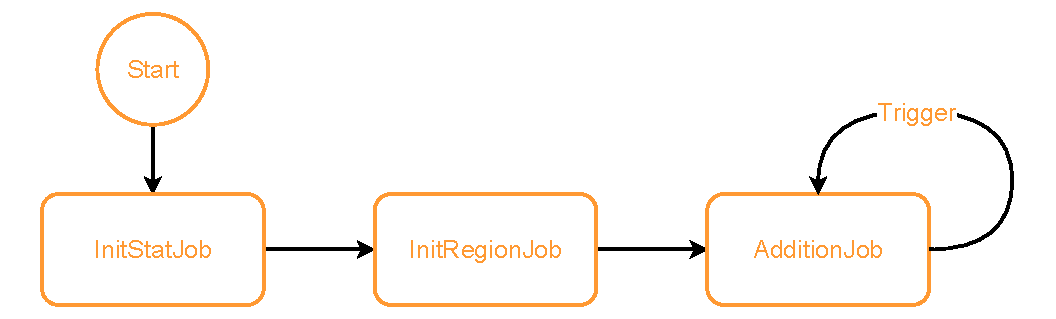
\includegraphics[width=\textwidth]{figures/jobs_scheduled.pdf}
\end{figure}

Při startu aplikace se spustí job \texttt{InitStatAzZsj}, až úspěšně skončí,
spustí se job \texttt{InitRegion}. Pokud je v konfiguraci nastaveno, že se job 
přeskočí tak job stále provede a dokončí jen bez zpracování dat.
Stejně to platí pro job \texttt{InitRegionJob}.
Problémem bylo, že job \texttt{InitStatAzZsj} a~\texttt{Additions} 
se spouštěly vždy při startu aplikace, protože měly trigger pro start. 
Ovšem job \texttt{Additions} se má spustit až po úspěšném dokončení jobu 
\texttt{InitRegion}. Tento problém bzl vyřešen pomocí \textbf{Semaforu}.
Konkrétně byl použit \texttt{Semaphore} z~balíčku \texttt{java.util.concurrent}.
Vzhledem k~tomu, že Quartz Scheduler má pro každý job vlastní vlákno,
je možné použít \texttt{Semaphore} pro zajištění, že se job \texttt{Additions}
může spustit až po úspěšném dokončení jobu \texttt{InitRegion}.

Semafor je inicializován na hodnotu 0, což znamená, že job \texttt{Additions}
se nemůže spustit, dokud není semafor uvolněn. Ten je uvolněn následně na konci 
jobu \texttt{InitRegion}. Jakmile se job \texttt{Additions} spustí poprvé, je pak 
opakovaně spouštěn podle nastavení cron v~konfiguračním souboru.

\subsubsection*{Semafor}
Semafor je synchronizační primitivum, které umožňuje řídit přístup 
k~sdíleným prostředkům v~multithreadovém prostředí.
Semafor může být binární (0 nebo 1) nebo počítací (libovolné celé číslo).
Následně má dvě hlavní operace:
\begin{itemize}
    \item \texttt{V()} -- uvolnění semaforu, zvýšení hodnoty semaforu o~1.
    \item \texttt{P()} -- zablokování semaforu, snížení hodnoty semaforu o~1, pokud je hodnota semaforu 0, vlákno se zablokuje a~čeká na uvolnění semaforu.
\end{itemize}

Tyto dvě operace jsou atomické, což znamená, že jsou prováděny jako jedna operace a~nelze je přerušit.
V Javě je semafor implementován pomocí třídy \texttt{Semaphore} z~balíčku \texttt{java.util.concurrent}.
P a V operace jsou implementovány jako metody \texttt{acquire()} a~\texttt{release()}.
Více o semaforech a~jeho použití je popsáno v~\cite{pesicka_semafor}. 



\section{Získávání dat z~API}
Stahování dat z~API RÚIAN je realizováno pomocí tříd \texttt{VdpClient} a~\texttt{VdpDownload},
které jsou součástí modulu \texttt{download}.

\subsection{VdpDownload}
Třída~\texttt{VdpDownload} se stará o~nastavení HTTP klienta~s~důvěrou ke všem certifikátům.
Využívá se zde knihovna~\texttt{Apache HttpClient}, která je součástí Spring Boot.
V~rámci metody \texttt{init()} se konfiguruje \texttt{SSLContext}, časové limity a~případně HTTP proxy.
Výsledný klient je uložen do proměnné \texttt{client}, která se následně používá pro volání metod \texttt{tryGet()} a~\texttt{trySaveFilter()}.
Tyto metody slouží ke stažení dat ze serveru VDP nebo k~inicializaci filtru pomocí HTTP požadavku.
Před ukončením aplikace je klient uzavřen pomocí metody označené anotací \texttt{@PreDestroy}.

\subsection{VdpClient}
\texttt{VdpClient} je hlavní komponenta~pro komunikaci se službou Veřejného dálkového přístupu (VDP).
Využívá celkem tři URL pro přístup k~seznamům souborů a~další tři URL pro stahování jednotlivých datových listů.
Adresy jsou většinou nastaveny v~konstantách této třídy, s~výjimkou jedné, která si URL generuje dynamicky podle data~předchozího dne.
Pro samotné stahování dat používá instanci třídy \\ \texttt{VdpDownload}.
Třída~obsahuje především tři metody, které jsou volány z~dříve popsaných \texttt{jobů}:
\begin{itemize}[itemsep=0pt]
    \item \texttt{zpracovatStatAzZsj()} -- zpracovává pouze jeden konkrétní soubor, se základními územními prvky,
    \item \texttt{getListLinksObce()} -- zpracovává sadu souborů, které obsahují seznamy obcí podle jednotlivých krajů,
    \item \texttt{getAdditions()} -- generuje datum pro přírůstková data a~stahuje soubor s~přírůstkovými daty.
\end{itemize}

Každá z~těchto metod nejprve stáhne textový soubor, který obsahuje seznam dostupných datových souborů.
Tento seznam se následně parsuje a~získané odkazy se využijí ke stažení souborů.
Metody \texttt{zpracovatStatAzZsj()} a~\texttt{getAdditions()} stahují pouze jeden konkrétní soubor,
zatímco \texttt{getListLinksObce()} stahuje všechny soubory dostupné v~seznamu.

Z~tohoto důvodu byla~doplněna~metoda~\texttt{downloadFilesFromLinks()}, která umožňuje stáhnout všechny soubory uvedené v~daném seznamu.
Získaná data~jsou obvykle ve formátu ZIP, jsou automaticky rozbalena~a~předána~jako \texttt{InputStream} dalším komponentám
prostřednictvím funkčního rozhraní \texttt{Consumer}.

Třída~rovněž implementuje opakování požadavků v~případě selhání, logování a~čištění dočasných souborů.

\section{Zpracování dat}
Jak bylo zmíněno výše, data~jsou zpracovávána~pomocí třídy \texttt{VdpClient}
a~pomocí funkčního rozhraní \texttt{Consumer} se předávají dalším komponentám.
A~to právě komponentě \texttt{VdpParser}, která se stará o~parsování XML souboru v předaném \texttt{InputStream}
a~následné ukládání do databáze.

Na~začátku se inicializuje \texttt{XMLStreamReader}, který se stará o~parsování XML souboru.
Reader je vytvořen pomocí třídy \texttt{XMLInputFactory}, která je součástí \\ knihovny \texttt{StAX}.

Původně byl použit \texttt{DocumentBuilder}, ale ten byl nahrazen \texttt{StAX} parserem.
Celé soubory si nejprve načítal do paměti a~poté je parsoval, po prvcích (\texttt{Node}).
To bylo v~případě malých souborů (příklad při zpracování malých obcí).
Problém nastal při zpracování velkých souborů (např. obec Praha),
Soubor dosahoval velikosti přes 1 GB a~bylo potřeba~jej zpracovat po částech.
Je ale velmi náročné dělit XML bez rozbití struktury souboru.
Proto se později přešlo na~\texttt{StAX} parser, který zpracovává XML po prvcích a~nepotřebuje celou strukturu XML.
\texttt{StAX} parser je mnohem efektivnější a~umožňuje zpracovávat velké soubory bez nutnosti načítat je celé do paměti.
Zároveň čte pouze události jako je začátek a~konec elementu, což je pro zpracování dat dostačující.
Stačí tedy nadefinovat jen název potřebných elementů a~tyto elementy parsovat.
U \texttt{DocumentBuilderu} bylo třeba~číst všechny Listy a~poté je zpracovávat.

\subsection{Parsing dat}
Jak už bylo řečeno výše, data~jsou parsována~ve třídě \texttt{VdpParser} s použitím \\ \texttt{XMLStreamReader}.
Zároveň ve stejném modulu se nachází i~třída~\texttt{VdpParserConsts}, která obsahuje konstanty pro názvy jednotlivých elementů.
Při čtení XML se nejprve čte hlavička~souboru. Ta~obsahuje nepotřebné informace, které se ignorují.
Dále se čtou jednotlivá data~počínající elementem \texttt{vf:Data}.
Nejprve je potřeba~ale rozeznat o jaký element se jedná (viz. \ref{tab:xmlStreamReader}).
\texttt{XMLStreamReader} rozeznává několik eventů a~u~každého eventu se provádí jiná akce a~získává jiná informace.

Příkladem, pokud se vyskytne event \texttt{START\_ELEMENT}, tak z~něj můžu získat název elementu a~jeho atributy.
Pokud se vyskytne event \texttt{CHARACTERS}, tak z~něj získám text uvnitř elementu, ale pokud se pokusím získat jméno elementu vyhodí to výjimku.

Cílem je tedy číst data~v cyklu, dokud nenarazím na~konec elementu \texttt{vf:Data}.
V průběhu čtení se nachází další důležité elementy, které určují, co se zrovna~čte za~objekt.
Jeden soubor může rozeznávat až 19 různých objektů, které se parsují do různých DTO objektů.
Každý jeden objekt podléhá jinému seznamu objektů.
Je tedy potřeba rozeznat, kdy začíná list a~kdy jeden objekt \ref{tab:seznamObjektu}.

\begin{table}[!h]
    \label{tab:xmlStreamReader}
    \centering
    \caption{Eventy XMLStreamReader}
    \begin{tabular}{|l|c|c|c|}
    \hline
    \multicolumn{1}{|c|}{\textbf{Event}} & \textbf{Hodnota~Event} & \textbf{Důležitá informace} & \textbf{Příklad}                                 \\ \hline
    \textit{START\_ELEMENT}              & 1                      & Název Elementu              & \textless{}vf:Data\textgreater{}                 \\ \hline
    \textit{END\_ELEMENT}                & 2                      & Název Elementu              & \textless{}/vf:Data\textgreater{} \\ \hline
    \textit{CHARACTERS}                  & 4                      & Hodnoty                     & Data~                                            \\ \hline
    \end{tabular}
\end{table}

\begin{table}[!h]
    \label{tab:seznamObjektu}
    \centering
    \caption{Seznam objektů a~jejich názvy}
    \begin{tabular}{|c|c|c|}
    \hline
    \textbf{Název}                       & \textbf{List Počátek/konec}                    & \textbf{Objekt Počátek/Konec}                 \\ \hline
    \textit{Stát}                        & \textless{}vf:Staty\textgreater{}              & \textless{}vf:Stat\textgreater{}              \\ \hline
    \textit{Region soudržnosti}          & \textless{}vf:RegionySourdznosti\textgreater{} & \textless{}vf:RegionSourdznosti\textgreater{} \\ \hline
    \textit{VÚSC}                        & \textless{}vf:Vusc\textgreater{}               & \textless{}vf:Vusc\textgreater{}              \\ \hline
    \textit{Okres}                       & \textless{}vf:Okresy\textgreater{}             & \textless{}vf:Okres\textgreater{}             \\ \hline
    \textit{ORP}                         & \textless{}vf:Orp\textgreater{}                & \textless{}vf:Orp\textgreater{}               \\ \hline
    \textit{POU}                         & \textless{}vf:Pou\textgreater{}                & \textless{}vf:Pou\textgreater{}               \\ \hline
    \textit{Obce}                        & \textless{}vf:Obce\textgreater{}               & \textless{}vf:Obec\textgreater{}              \\ \hline
    \textit{Spravní obvod}               & \textless{}vf:SpravniObvody\textgreater{}      & \textless{}vf:SpravniObvod\textgreater{}      \\ \hline
    \textit{MOP}                         & \textless{}vf:Mop\textgreater{}                & \textless{}vf:Mop\textgreater{}               \\ \hline
    \textit{MOMC}                        & \textless{}vf:Momc\textgreater{}               & \textless{}vf:Momc\textgreater{}              \\ \hline
    \textit{Část obce}                   & \textless{}vf:CastiObci\textgreater{}          & \textless{}vf:CastiObce\textgreater{}         \\ \hline
    \textit{Katastrální území}           & \textless{}vf:KatastralniUzemi\textgreater{}   & \textless{}vf:KatastralniUzemi\textgreater{}  \\ \hline
    \textit{Parcela}                     & \textless{}vf:Parcely\textgreater{}            & \textless{}vf:Parcely\textgreater{}           \\ \hline
    \textit{Ulice}                       & \textless{}vf:Ulice\textgreater{}              & \textless{}vf:Ulice\textgreater{}             \\ \hline
    \textit{Stavební objekt}             & \textless{}vf:StavebniObjekty\textgreater{}    & \textless{}vf:StavebniObjekt\textgreater{}    \\ \hline
    \textit{Adresní místo}               & \textless{}vf:AdresniMista\textgreater{}       & \textless{}vf:AdresniMisto\textgreater{}      \\ \hline
    \textit{ZSJ}                         & \textless{}vf:Zsj\textgreater{}                & \textless{}vf:Zsj\textgreater{}               \\ \hline
    \textit{VO}                          & \textless{}vf:VO\textgreater{}                 & \textless{}vf:VO\textgreater{}                \\ \hline
    \textit{Zaniklý prvek}               & \textless{}vf:ZaniklePrvky\textgreater{}       & \textless{}vf:ZaniklyPrvek\textgreater{}      \\ \hline
    \end{tabular}
\end{table}

\newpage

\begin{code}{XML}{Příklad struktury XML}{lst:vfStruktura}
<vf:Data>
    <vf:Staty>
        <sti:Stat>
            <sti:Kod>...</sti:Kod>
        </sti:Stat>
    </vf:Staty>
</vf:Data>
\end{code}

Každý element je rozdělen na~dvě části.
Klasifikátor a~název elementu.
Klasifikátor je určen pro rozlišení jednotlivých elementů a do jaké úrovně patří.
Podle názvu elementu se určuje jaký objekt se parsuje.
V příkladu \ref{lst:vfStruktura} je uveden \texttt{vf} klasifikátor (\textit{výměnný formát}), který je nejvyšší úrovní.
Každý seznam objektů využívá určitý klasifikátor, přičemž každý objekt má přiřazený vlastní, specifický klasifikátor.
Každý objekt dále obsahuje atributy, které odpovídají tomuto klasifikátoru.
Příkladem může být dvojice \texttt{vf:Stat} a~\texttt{sti:Kod},
kde \texttt{vf} je klasifikátor pro seznam států a~\texttt{sti} je klasifikátor pro stát.

V~případě, že je atribut cizím klíčem, používá se klasifikátor objektu, na který odkazuje.
Může se také vyskytnout atribut, který představuje další tabulku nebo seznam tabulek.
V~takovém případě se pro tyto tabulky používá klasifikátor \texttt{com}.
Příklady klasifikátorů jsou uvedeny v~příkladu \ref{lst:klasifikator}.

\begin{code}{XML}{Příklad Klasifikátorů}{lst:klasifikator}
<vf:Data>
    <vf:Okresy>
        <vf:Okres>
            <oki:Kod>100</oki:Kod>
            <oki:Nazev>...</oki:Nazev>
        </vf:Okres>
    </vf:Okresy>
    <vf:Obce>
        <vf:Obec>
            <obi:Kod>...</obi:Kod>
            <obi:Nazev>...</obi:Nazev>
            <obi:Okres>
                <oki:Kod>100<oki:Kod>
            </obi:Okres>
            <obi:MluvnickeCharakteristiky>
                <com:Pad2>...</com:Pad2>
                <com:Pad3>...</com:Pad3>
            </obi:MluvnickeCharakteristiky>
        </vf:Obec>
    </vf:Obce>
</vf:Data>
\end{code}

\subsection{Atributy Objektů}
V tabulce \ref{tab:datove_typy} byly zmíněné všechny datové typy a~jejich rozdíly mezi databázemi.
Podle dokumentace RÚIAN VFR \cite{ruian_vfr}, každý atribut objektu má také svůj datový typ.
Konkrétně se jedná o~tyto datové typy:
\begin{itemize}
    \item \textbf{String} -- textový řetězec, který může obsahovat písmena, číslice a~speciální znaky.
    \item \textbf{Integer} -- celé číslo bez desetinné části.
    \item \textbf{Long} -- reálné číslo s~desetinnou částí.
    \item \textbf{Boolean} -- logická hodnota, která může nabývat hodnoty true nebo false.
    \item \textbf{Binární data} -- binární data, která budou primárně obsahovat obrázky.
    \item \textbf{DateTime} -- datum a~čas ve formátu \texttt{YYYY-MM-DDTHH:MM:SS} (příklad: 2007-12-03T10:15:30).
    \item \textbf{Kolekce} -- seznam objektů nebo hodnot, které jsou uloženy v~jednom atributu.
\end{itemize}

Datové typy jako \texttt{String}, \texttt{Integer}, \texttt{Boolean} a~\texttt{Long} jsou standardní datové typy.
\texttt{DateTime} je datový typ, který se používá pro ukládání data~a~času.
Co se týče binárních dat, tak ty budou uloženy jako \texttt{byte[]},
ale aplikace tyto data~zatím nezpracovává.
Ovšem zmíněné \texttt{Kolekce} jsou označeny všechny atributy, které obsahují více hodnot nebo cizí klíče.
Kolekce budou do databáze ukládány jako \textbf{JSON}.

\subsubsection*{JSON Objekty}
Proč byly zvoleny JSON objekty? Tabulky dle specifikace nebyly vhodné pro rozdělení na~další tabulky a~vytváření cizích klíčů.
Některé kolekce totiž mohou být 1:1 nebo N:M. Proto byl zvolen JSON formát, který je vhodný pro ukládání takových to dat.
Některé kolekce jsou uloženy jako JSON Objekt a~některé jako JSON pole (Pole JSON Objektů).
Pro každou JSON kolekci byla vytvořena specifická JSON mapovací metoda. Každá tato metoda~funguje podobně jako XML parser.
Hledá elementy, které jsou uloženy v~kolekci a~převede je na~JSON objekt nebo pole.
Všechny atributy jednotlivých JSON objektů jsou uloženy v konstantách v~modulu \texttt{jsonObjects}.

\subsubsection*{Kolekce JSON Objekt}
Tyto kolekce vždy obsahují pouze jeden JSON Objekt.
Každá kolekce má svou vlastní metodu pro parsování.
Jedná se o~kolekce:
\begin{itemize}
    \item \textbf{Mluvnické Charakteristiky} -- metoda~\texttt{readMCh()},
    \item \textbf{Čísla~domovní} -- metoda~\texttt{readCislaDomovni()},
    \item \textbf{Nespravné Údaje} -- metoda~\texttt{readNespravneUdaje()},
\end{itemize}

\subsubsection*{Kolekce JSON Pole}
Tyto kolekce mohou obsahovat jednu nebo více Objektů.
Pro tyto kolekce se používá sada dvou metod. Jedna pro kolekci a~druhá pro jednotlivý objekt. 
Jedná se o kolekce:
\begin{itemize}
    \item \textbf{Bonitované díly / Bonitovaný díl} -- metoda~\texttt{readBonitovaneDily()} a~\texttt{readBonitovanyDil()},
    \item \textbf{Způsoby ochrany / Způsob ochrany} -- metoda~\texttt{readZpusobyOchrany()} a~\texttt{readZpusobOchrany()},
    \item \textbf{DetailniTEA} -- metoda~\texttt{readDetailniTeas()} a~\texttt{readDetailniTea()},
\end{itemize}

V přírůstkových datech se nachází i další kolekce, a~to \textbf{Nezjištěné údaje}.
Ta~je kompletně ignorována~a~neukládá se do databáze.

\subsubsection*{Kolekce s cizími klíči}
Cizí klíče jsou uloženy jako kolekce, které obsahují pouze jeden cizí klíč.
Z těchto kolekcí se tedy získává pouze Integer nebo Long.
Vzhledem k tomu, že se jedná o~cizí klíče, které odkazují na~jiné objekty,
byly vytvořeny metody pro parsování těchto cizích klíčů.
Metoda~\texttt{readFK()} a~\texttt{readFKLong} dostane jako parametr název elementu a~vrací Integer nebo Long.
Rozdělení na~Integer a~Long je z~důvodu, že je zde objekt \textbf{Parcela}, která má primární klíč jako Long.

\subsubsection*{Geometrie}
Geometrie je uložena~speciální kolekce obsahující až 3 možné geometrické údaje.
V základní datové sadě se nachází pouze Definiční bod specifikující střed daného objektu na~mapě.
V rozšířených se pak dodatečně nachází i~Generalizované Hranice a~Originální Hranice.
Je zde i~případ Definiční čáry, která je uložena~jako \texttt{LineString} nebo \texttt{MultiLineString}.
Tato geometrie se vyskytuje pouze u objektů \textbf{Ulice}.
O problematiku parsování geometrie se stará třída~\texttt{GeometryParser} v~modulu \texttt{geometry}, která parsuje jednotlivé geometrické objekty.
V současné práci se řeší pouze Definiční bod, který je uložen jako \texttt{Point} nebo \texttt{MultiPoint}.
Generalizované Hranice a~Originální Hranice jsou uloženy jako \texttt{Polygon} nebo \texttt{MultiPolygon}.
Stejně jako u~JSON objektů i~geometrie se čte podle eventu a~atributů v elementu.
Názvy geometrických objektů jsou uloženy jako konstanty v modulu \texttt{geometryParserConsts} s příslušným jménem k objektu.
Výstupem všech metod pro parsování geometrie je \texttt{Geometry} objekt z~knihovny \texttt{JTS}.

\newpage

\subsection{Ukládání dat do databáze}
Po úspěšném parsování jedné sady objektů (např. \textbf{Obce}) nám vznikne list Dto objektů
dané sady, které se následně ukládají do databáze. Tento list se následně předává do metody \texttt{prepareAndSave()},
která se nachází v~příslušné service třídě (např. \texttt{ObecService}) \ref{sec:serviceTridy}.
Tato metoda se stará o~přípravu a uložení dat do databáze.
Metoda není použita v~případě, pokud je v~konfiguraci nastaveno \texttt{howToProcess} na~\texttt{selected}
a~není v~konfiguraci uvedena~tabulka~daného objektu.

Jak metoda~\texttt{prepareAndSave()} funguje?
Pro každý objekt se provede několik kontrol a~úprav.

\begin{itemize}
    \item \textbf{Bezpečnostní kontrola} -- slouží k~zabránění chyby nebo neplatným datům v~databázi.
    \item \textbf{Úprava~dat} -- slouží k~úpravě dat podle konfigurace a~podle již existujících dat v~databázi.
\end{itemize}

\begin{enumerate}
    \item \textit{(Bezpečnostní kontrola)} Pokud objekt neobsahuje primární klíč, kontrola~se zastaví a~po 
    zpracování všech objektů bude odstraněn ze seznamu.
    
    \item \textit{(Úprava~dat)} Když se objekt, již nachází v~databázi:
    \begin{enumerate}
        \item Pokud je v~konfiguraci u~tabulky nastaveno \texttt{howToProcess} na~\texttt{all}:
        Pokud je atribut u~nového objektu \texttt{null} a~v~databázi je \texttt{notnull}, tak se použije hodnota~z~databáze.
        \item Pokud je v~konfiguraci u~tabulky nastaveno \texttt{howToProcess} na~\texttt{include}:
        Pokud je atribut u~nového objektu atribut \texttt{notnull} a~v~konfiguraci tento atribut není uveden, tak se použije hodnota~z~databáze,
        jinak se použije hodnota~z~nového objektu.
        \item Pokud je v~konfiguraci u~tabulky nastaveno \texttt{howToProcess} na~\texttt{exclude}:
        Pokud je atribut u~nového objektu atribut \texttt{notnull} a~v~konfiguraci tento atribut je uveden, tak se použije hodnota~z~databáze,
        jinak se použije hodnota~z~nového objektu.
    \end{enumerate}

    \item \textit{(Úprava~dat)} Když se objekt ještě nenachází v~databázi:
    \begin{enumerate}
        \item Pokud je v~konfiguraci u~tabulky nastaveno \texttt{howToProcess} na~\texttt{all}:
        Objekt se uloží do databáze tak jak je bez dodatečných úprav.
        \item Pokud je v~konfiguraci u~tabulky nastaveno \texttt{howToProcess} na~\texttt{include}:
        Objektu se dá hodnota~null u~atributů, které nejsou uvedeny v~konfiguraci.
        \item Pokud je v~konfiguraci u~tabulky nastaveno \texttt{howToProcess} na~\texttt{exclude}:
        Objektu se dá hodnota~null u~atributů, které jsou uvedeny v~konfiguraci.
    \end{enumerate}

    \item \textit{(Bezpečnostní kontrola)} Ověří, zda~objekt obsahuje cizí klíč, ověří se jeho platnost a~existence v~databázi.
    Pokud cizí klíč neexistuje, kontrola~se zastaví a~objekt se přidá na list pro odstranění a~po zpracování všech objektů
    bude odstraněn ze seznamu.
\end{enumerate}

Úprava~dat má dvě verze podle toho, zdali se jedná o~nový nebo již existující objekt.
Objekt z~databáze se vybírá selekcí podle primárního klíče.
Do paměti se načte objekt z~databáze a~podle toho se upraví nový objekt.

Během těchto kontrol se také loguje, kolik prvků z~listu bylo zpracováno.
Jedná se o~milníky \textit{25 \%}, \textit{50 \%}, \textit{75 \%} a~\textit{100 \%}.

Po úspěšném zpracování listu objektů se vypíše, kolik objektů bylo odstraněno a~nebude uloženo do databáze.

Pak přijde na~řadu ukládání dat do databáze.
To probíhá tak, že si list objektů rozdělí na~menší části podle velikosti \texttt{commitSize} z~konfigurace nebo menší.
Tento list se pak následně uloží do databáze pomocí metody \texttt{saveAll()}.

\section{Po zpracování dat}
Jakmile jsou data~úspěšně přečtena~a~uložena~do databáze, je potřeba~provést další úkony.
Ve třídě \texttt{VdpClient} u~metody \texttt{unzipContent()} se po úspěšném rozbalení souboru
a~zpracování souboru v~try bloku nachází finally blok který se postará o~smazaní dočasného souboru.
Tento blok se vykoná i~v~případě, že dojde k~výjimce a~soubor se neuloží do databáze.

Jakmile se soubor úspěšně vymaže z~disku může začít nový job nebo zpracování dalšího souboru
v~případě, že se jedná o~job \texttt{InitRegionJob}. 
Dále po zpracování regionů se zpracují přírůstková data (job \texttt{AdditionJob})

\chapter{Testování}
\section{Rychlostní porovnání databázových systémů}
Tento test byl proveden na stejném konfiguračním souboru pro všechny databázové systémy.
Testovací konfigurace je nastavena na provedení stažení, zpracování a~uložení Základní datové sady Stát~až~ZSJ.
Tato datová sada byla vybrána z důvodu neměnnosti. 
Data v této datové sadě se mění jen velmi zřídka a~je možné je stáhnout.
Dále bylo nastavené, že se zpracují všechny tabulky uvedené v~již zmíněné datové sadě.
Geometrie bude zpracována a~velikost jednotlivých commitů bude 2000.
Vzhled konfiguračního souboru je uveden v~příkladu \ref{lst:konfigTest} a~bude konfigurován pro PostgreSQL.
Testování probíhalo na stejném stroji, který měl instalované všechny databázové systémy.

Nad všemi databázovými systémy probíhaly testy \(3\times\), aby se eliminovaly chyby způsobené jinými procesy na serveru.
Každý test byl proveden na prázdné databázi.
Měření začalo, když byla data připravena ke čtení z důvodu eliminace stahování dat z~internetu.
Konkrétně když se vypsala zpráva \uv{Data proccesing started.} a~následně skončilo, když se 
vypsala zpráva \uv{Data proccesing finished.}.
Během tohoto testu byl také vyfiltrováno 1 ZSJ z důvodu neexistence cizího klíče v~tabulce Katastrální území.
Testování proběhlo s daty \url{https://vdp.cuzk.gov.cz/vymenny_format/soucasna/20250331_ST_UZSZ.xml.zip}
Výsledky jsou uvedeny v~tabulce \ref{tab:test1} a mají formát HH:MM:SS.

\begin{table}[!h]
  \centering
  \caption{Časy testů pro používané databáze}
  \label{tab:test1}
  \begin{tabular}{|c|c|c|c|}
  \hline
                  & \textbf{PostgreSQL} & \textbf{MS SQL} & \textbf{Oracle} \\ \hline
  \textbf{test 1} & 0:35:59             & 0:22:46         & 1:04:19         \\ \hline
  \textbf{test 2} & 0:37:03             & 0:22:26         & 1:05:30         \\ \hline
  \textbf{test 3} & 0:35:53             & 0:21:26         & 1:04:57         \\ \hline
  \textbf{průměr} & 0:36:18             & 0:22:13         & 1:04:55         \\ \hline
  \end{tabular}
\end{table}

Jak je vidět v tabulce \ref{tab:test1}, ukázalo se že MS SQL je nejrychlejší databázový systém pro zpracování datové sady.
PostgreSQL je o~přesně 14 minut pomalejší než MS SQL a~Oracle je o~přesně 28 minut pomalejší než MS SQL.
Je ale možné že Oracle je pomalejší z důvodu že se jedná o~Express verzi, která je omezena na 2GB RAM a~1 CPU.
Dále je možné že rychlost byla omezena prostředím. Zatím co PostgreSQL a MS SQL běžely v Docker kontejneru, 
Oracle běžel přímo na hostitelském systému.

\begin{lstlisting}[language=json, caption={Konfigurační soubor pro test rychlosti}, label={lst:konfigTest}]
    {
        "database": {
          "type": "postgresql",
          "url": "jdbc:postgresql://localhost:5432",
          "dbname": "ruian",
          "username": "postgres",
          "password": "123"
        },
        "quartz": {
          "cron": "0 0 2 * * ?",
          "skipInitialRunStat": false,
          "skipInitialRunRegion": true
        },
        "vuscCodes": {},
        "additionalOptions": {
          "includeGeometry": true,
          "commitSize": 2000
        },
        "dataToProcess": {
          "howToProcess": "all"
        }
      }    
\end{lstlisting}


\section{Testování kompletního importu}


\chapter{Budoucí rozšíření a úpravy}
Na této aplikaci je stále co přidávat, vylepšovat a~upravit.
Proto se v následujících sekcích pokusím shrnout, co by se 
dalo do budoucna vylepšit a přidat.

\section*{Uživatelské rozhraní}
Jediný uživatelský pohled na aplikaci je v~současnosti zajištěn pomocí 
logu, který je generován v~textovém formátu. Jedná se pouze o výpis
informací o~prováděných úkonech, které aplikace dělá.
Bylo by dobré přidat uživatelské rozhraní, které by bylo schopné
zobrazit informace o~prováděných úkonech v~reálném čase.


\section*{Optimalizace}
Aplikace je v~současnosti napsána tak, že se snaží aby byla schopná
zpracovat jakákoliv data z~RÚIANu. Ovšem rychlostně to není
úplně ideální. Hlavním kamenem úrazu je především kontrola
a~porovnání nových dat s~těmi, které jsou už v~databázi.
Bylo by dobré nějak zefektivnit tento proces, aby se obecně zrychlil
celý proces zpracování dat.

\section*{Refektoring kódu}
Tenhle oddíl vzchází trochu z~předchozího. Aplikace je napsána
tak aby byla schopná zpracovat jakákoliv data z~RÚIANu.
Bylo bz proto dobré udělat refaktoring kódu, aby se zjednodušil
a zefektivnil celý proces zpracování dat. Service třídy, Dto 
by se určitě upravit pomocí nějakého generického rozhraní.
Využití abstraktních tříd a~rozhraní by mělo celý kód velmi
zjednodušit.

\section*{Zpracování zbylých dat}
V současnosti aplikace zpracovává pouze základní datové sady.
To znamená zpracování zbývajících geometrických dat, které jsou
v~RÚIANu k~dispozici. Dále zakomponovat obrázky (binární data),
které se u některých objektů vyskytují.
Databáze je v~současnosti připravena na zpracování těchto dat,
ale aplikace nemá implementovanou logiku pro jejich zpracování.

\section*{Podpora pro dalších databázových systémů}
Rozšíření aplikace o~další databázové systémy by bylo mohla
býti samozřejmostí. V~současnosti je aplikace napsána tak,
že je schopná pracovat pouze s~PostgreSQL, MS SQL a~Oracle databázemi.
Bylo by dobré přidat podporu pro další databázové systémy.

\chapter{Závěr}
Hlavním cílem této bakalářské práce bylo vytvořit aplikaci, která by byla
schopná stahovat data podle konfigurace z~RÚIANu a~ukládat je do databáze.
V rámci práce jsem navrhl prvotní verzi aplikace, která splňuje tento cíl,
implementoval jsem ji a~otestoval jsem ji na vzorových datech z~RÚIANu
pro všechny zadané databázové systémy.

Vytvořená aplikace je první verze aplikace se jménem \textbf{Ruian\_Puller},
která má za úkol stahovat data z~RÚIANu a~ukládat je do databáze.
Podporované databáze jsou PostgreSQL, MySQL a~Oracle.
Aplikace je napsaná v~programovacím jazyce Java a~využívá framework Spring Boot.
Je možné použití plánování úloh pomocí Quartz Scheduleru.
Aplikace se nastavuje podle konfiguračního souboru,
který je ve formátu JSON. Nastavuje se připojení k databázi,
jaké prvky se mají stahovat, či ignorovat a~jak často se stahování má provádět.
Aplikace je navržena jako základ pro budoucí rozšíření a úpravy (viz kapitola~\ref{cha:NavrhDoBudoucna}).
 
%1--------------------------------------------------------------------------

\appendix

%2--------------------------------------------------------------------------
\chapter{Uživatelská příručka}
\section*{Co je to Ruian Puller?}
Tato aplikace stahuje data z~\url{https://vdp.cuzk.cz/vdp/ruian/vymennyformat} a~ukládá je do~SQL databáze.
Podporované databáze:
\begin{itemize}
  \item \textbf{Microsoft SQL}
  \item \textbf{PostgreSQL}
  \item \textbf{Oracle}
\end{itemize}

Data jsou stahována ve formátu XML a~převáděna do~DTO (Data Transfer Object), které jsou následně ukládány do~databáze pomocí JPA (Java Persistence API).\\
Aplikace je napsána v~Javě~21 a~používá Spring Boot pro snadné nastavení a~konfiguraci. Všechny závislosti jsou spravovány pomocí Maven.\\
Aplikace dokáže stahovat a~ukládat standardní datové sady:
\begin{itemize}
  \item Stát až ZSJ (základní)
  \item Všechny kraje a~obce (základní)
  \item Přírůstková data (základní)
\end{itemize}

\section*{Před prvním spuštěním}
Je třeba mít zprovozněné SQL databáze pro ukládání dat. Databáze může běžet podle vlastních nastavení, nebo lze použít variantu s~Dockerem.
V~adresáři \texttt{database} se nachází podadresáře pro každou z~podporovaných databází. Každý podadresář obsahuje \texttt{docker-compose.yml} a~\texttt{init.sql},
které vytvoří databázi a~tabulky pro ukládání dat.
Oracle databáze neobsahuje \texttt{docker-compose.yml}, protože byla vytvořena mimo Docker.

\subsection*{Docker MS SQL a~PostgreSQL}
Pro spuštění v~Dockeru je zde adresář \texttt{db}, kde jsou dva podadresáře: PostgreSQL a~MS SQL. V~každém je příslušný \texttt{docker-compose.yml} a~\texttt{init.sql}.

Pro vytvoření instancí spusťte v~příslušném adresáři:
\begin{lstlisting}[language=bash]
docker-compose up -d
\end{lstlisting}

Pro případné vyčištění:
\begin{lstlisting}[language=bash]
docker-compose down -v
\end{lstlisting}

\subsection*{Oracle}
Oracle databáze je vytvořena mimo Docker. Je třeba mít nainstalovanou Oracle Database 19c nebo vyšší. Pro vytvoření instance použijte \texttt{init.sql}.
Chování databáze je následně stejné jako u~předchozích dvou.

\section*{Aplikace}
Aplikace se nachází v~adresáři \texttt{app}, kde je zdrojový kód a~Maven projekt. Je napsána v~Javě~21 a~používá Spring Boot. Závislosti jsou spravovány pomocí Maven.
Projekt je nastaven na~JDK~21 a~Maven~3.8.6 a~je spustitelný v~IntelliJ IDEA nebo Eclipse.

\section*{Konfigurace}
Konfigurační soubor \texttt{config.json} obsahuje nastavení připojení k~databázi, seznam tabulek a~další volby. Nachází se v~adresáři \texttt{src/main/resources}.

\newpage

\begin{lstlisting}[language=json, caption={Příklad konfiguračního souboru}]
{
  "database": {
    "type": "<databse_type>",
    "url": "<connection_string>",
    "dbname": "<database_name>",
    "username": "<username>",
    "password": "<password>"
  },
  "quartz": {
    "cron": "0 0 2 * * ?",
    "skipInitialRunStat": false,
    "skipInitialRunRegion": true
  },
  "vuscCodes": {
    "<kod>": "<kraj_nazev>"
  },
  "additionalOptions": {
    "includeGeometry": true,
    "commitSize": 1000
  },
  "dataToProcess": {
    "howToProcess": "<all/selected>",
    "tables": {
      "<tablename>": {
        "howToProcess": "<all,include,exclude>",
        "columns": ["<column_name>", "<column_name>", ...]
      }
    }
  }
}
\end{lstlisting}

\newpage

\subsection*{Popis jednotlivých částí}
\begin{itemize}
  \item \textbf{database} -- nastavení připojení k~databázi:
  \begin{itemize}
    \item \texttt{type}: typ databáze (postgresql, mssql, oracle)
    \item \texttt{url}: connection string
    \item \texttt{dbname}, \texttt{username}, \texttt{password}
  \end{itemize}

  \item \textbf{quartz} -- plánovač stahování dat:
  \begin{itemize}
    \item \texttt{cron}: výraz pro plánovač
    \item \texttt{skipInitialRunStat} -- přeskočit inicializaci Stát až ZSJ (true/false)
    \item \texttt{skipInitialRunRegion} -- přeskočit inicializaci krajů (true/false)
  \end{itemize}

  \item \textbf{vuscCodes} -- kódy krajů a~obcí:
  \begin{longtable}{|c|c|}
    \caption{Seznam krajů a~jejich kódů} \\
    \hline
    \textbf{Kód} & \textbf{Kraj} \\
    \hline
    19 & Hlavní město Praha \\
    27 & Jihočeský kraj \\
    35 & Jihomoravský kraj \\
    43 & Karlovarský kraj \\
    51 & Kraj Vysočina \\
    60 & Královéhradecký kraj \\
    78 & Liberecký kraj \\
    86 & Moravskoslezský kraj \\
    94 & Olomoucký kraj \\
    108 & Pardubický kraj \\
    116 & Plzeňský kraj \\
    124 & Středočeský kraj \\
    132 & Ústecký kraj \\
    141 & Zlínský kraj \\
    \hline
  \end{longtable}

  \newpage

  \item \textbf{additionalOptions} -- další volby:
  \begin{itemize}
    \item \texttt{includeGeometry} -- zahrnout geometrii (true/false)
    \item \texttt{commitSize} -- velikost dávky pro commit (default 1000)
  \end{itemize}

  \item \textbf{dataToProcess} -- nastavení pro zpracování dat:
  \begin{itemize}
    \item \texttt{howToProcess} -- jak zpracovat data (all/selected)
    \item \texttt{tables} -- nastavení pro jednotlivé tabulky:
    \begin{itemize}
      \item \texttt{howToProcess} -- jak zpracovat tabulku (all/include/exclude)
      \item \texttt{columns} -- seznam sloupců pro zpracování
    \end{itemize}
  \end{itemize}
\end{itemize}

\begin{center}
  \begin{longtable}{|>{\raggedright\arraybackslash}p{4cm}|>{\raggedright\arraybackslash}p{9cm}|}
    \caption{Seznam tabulek a sloupců} \\

    \hline
    \textbf{Tabulka} & \textbf{Sloupce} \\
    \hline
    \endfirsthead
    
    \hline
    \textbf{Tabulka} & \textbf{Sloupce} \\
    \hline
    \endhead
  
    stat & nazev, nespravny, platiod, platido, idtransakce, globalniidnavrhuzmeny, nutslau, geometriedefbod, geometriegenhranice, geometrieorihranice, nespravneudaje, datumvzniku \\
    \hline
    regionSoudrznosti & nazev, nespravny, stat, platiod, platido, idtransakce, globalniidnavrhuzmeny, nutslau, geometriedefbod, geometriegenhranice, geometrieorihranice, nespravneudaje, datumvzniku \\
    \hline
    vusc & nazev, nespravny, regionsoudrznosti, platiod, platido, idtransakce, globalniidnavrhuzmeny, nutslau, geometriedefbod, geometriegenhranice, geometrieorihranice, nespravneudaje, datumvzniku \\
    \hline
    okres & nazev, nespravny, kraj, vusc, platiod, platido, idtransakce, globalniidnavrhuzmeny, nutslau, geometriedefbod, geometriegenhranice, geometrieorihranice, nespravneudaje, datumvzniku \\
    \hline
    orp & nazev, nespravny, spravniobeckod, vusc, okres, platiod, platido, idtransakce, globalniidnavrhuzmeny, geometriedefbod, geometriegenhranice, geometrieorihranice, nespravneudaje, datumvzniku \\
    \hline
    pou & nazev, nespravny, spravniobeckod, orp, platiod, platido, idtransakce, globalniidnavrhuzmeny, geometriedefbod, geometriegenhranice, geometrieorihranice, nespravneudaje, datumvzniku \\
    \hline
    obec & nazev, nespravny, statuskod, okres, pou, platiod, platido, idtransakce, globalniidnavrhuzmeny, mluvnickecharakteristiky, vlajkatext, vlajkaobrazek, znaktext, znakobrazek, clenenismrozsahkod, clenenismtypkod, nutslau, geometriedefbod, geometriegenhranice, geometrieorihranice, nespravneudaje, datumvzniku \\
    \hline
    castObce & nazev, nespravny, obec, platiod, platido, idtransakce, globalniidnavrhuzmeny, mluvnickecharakteristiky, geometriedefbod, nespravneudaje, datumvzniku \\
    \hline
    mop & nazev, nespravny, obec, platiod, platido, idtransakce, globalniidnavrhuzmeny, geometriedefbod, geometrieorihranice, nespravneudaje, datumvzniku \\
    \hline
    spravniObvod & nazev, nespravny, spravnimomckod, obec, platiod, platido, idtransakce, globalniidnavrhuzmeny, geometriedefbod, geometrieorihranice, nespravneudaje, datumvzniku \\
    \hline
    momc & nazev, nespravny, spravniobvod, mop, obec, spravniobvod, platiod, platido, idtransakce, globalniidnavrhuzmeny, vlajkatext, vlajkaobrazek, znaktext, znakobrazek, mluvnickecharakteristiky, geometriedefbod, geometrieorihranice, nespravneudaje, datumvzniku \\
    \hline
    katastralniUzemi & nazev, nespravny, existujedigitalnimapa, obec, platiod, platido, idtransakce, globalniidnavrhuzmeny, rizeniid, mluvnickecharakteristiky, geometriedefbod, geometriegenhranice, nespravneudaje, datumvzniku \\
    \hline
    parcela & nespravny, kmenovecislo, pododdelenicisla, vymeraparcely, zpusobyvyuzitipozemku, druhcislovanikod, druhpozemkukod, katastralniuzemi, platiod, platido, idtransakce, rizeniid, bonitovanedily, zpusobyochranypozemku, geometriedefbod, geometrieorihranice, nespravneudaje \\
    \hline
    ulice & nazev, nespravny, obec, platiod, platido, idtransakce, globalniidnavrhuzmeny, geometriedefbod, geometriedefcara, nespravneudaje \\
    \hline
    stavebniObjekt & cislodomovni, identifikacniparcela, typstavebnihoobjektukod, castobce, momc, platiod, platido, idtransakce, globalniidnavrhuzmeny, isknbudovaid, dokonceni, druhkonstrukcekod, obestavenyprostor, pocetbytu, pocetpodlazi, podlahovaplocha, pripojenikanalizacekod, pripojeniplynkod, pripojenivodovodkod, vybavenivytahemkod, zastavenaplocha, zpusobvytapenikod, zpusobyochrany, detailnitea, geometriedefbod, geometrieorihranice, nespravneudaje \\
    \hline
    adresniMisto & nespravny, cislodomovni, cisloorientacni, cisloorientacnipismeno, psc, stavebniobjekt, ulice, vokod, platiod, platido, idtransakce, globalniidnavrhuzmeny, geometriedefbod, nespravneudaje \\
    \hline
    zsj & nazev, nespravny, katastralniuzemi, platiod, platido, idtransakce, globalniidnavrhuzmeny, mluvnickecharakteristiky, vymera, charakterzsjkod, geometriedefbod, geometriegenhranice, geometrieorihranice, nespravneudaje, datumvzniku \\
    \hline
    vo & platiod, platido, idtransakce, globalniidnavrhuzmeny, geometriedefbod, geometriegenhranice, geometrieorihranice, nespravneudaje, cislo, nespravny, obec, momc, poznamka \\
    \hline
    zaniklyPrvek & typprvkukod, idtransakce \\
    \hline
    
  \end{longtable}
\end{center}

\textit{Poznámky:}
\begin{enumerate}
  \item Quartz Scheduler obsahuje dvě boolean nastavení pro přeskočení kroků inicializace.
  \item Všechny tabulky kromě \texttt{vo} byly testovány. Je tedy možné, že při parsování dojde k~chybě.
\end{enumerate}

\section*{Průběh aplikace}
\begin{enumerate}
  \item Aplikace načte nastavení z~\texttt{config.json}.
  \item Pokud je \texttt{skipInitialRunStat = false}, stáhne se Stát až ZSJ.
  \item Pokud je \texttt{skipInitialRunRegion = false}, stáhnou se vybrané kraje.
  \item Následně se stahují přírůstková data.
  \item Aplikace čeká na~další běh dle Quartz Scheduleru.
\end{enumerate}

Aplikace nepřepisuje data, pouze přidává nové nebo aktualizuje existující záznamy.
Pokud nastane chyba typu Foreign Key, problémový objekt se přeskočí a~pokračuje se dál.

\chapter{Struktura přiloženého zip souboru}
\begin{forest}
  for tree={
    font=\ttfamily,
    grow'=0,
    child anchor=west,
    parent anchor=south,
    anchor=west,
    calign=first,
    s sep=5pt,
    l sep=10pt,
    edge path={
      \noexpand\path [draw, \forestoption{edge}]
      (!u.south west) +(7.5pt,0) |- node[fill,inner sep=1.25pt] {} (.child anchor)\forestoption{edge label};
    },
    before typesetting nodes={
      if n=1
        {insert before={[,phantom]}}
        {}
    },
    fit=band,
    before computing xy={l=15pt},
  }  
[
  [Aplikace\_a\_knihovny \dotfill{........} Zdrojové kódy + aplikace a JavaDoc
    [src \dotfill{..................................} Zdrojové kódy aplikace]
    [pom.xml \dotfill{.......................................} Maven pom.xml]
    [Ruian\_Puller-1.jar \dotfill{.............................} Runnable JAR]
    [Java\_Doc \dotfill{............................................} JavaDoc]
  ]
  [Text\_prace \dotfill{...............................} Text práce + přílohy
    [textSrc \dotfill{.................................} Zdrojové kódy testu]
    [figures \dotfill{.............................................} Obrázky]
    [bib.bib \dotfill{........................................} Bibliografie]
    [doc.tex \dotfill{.........................................} Hlavní text]
    [Bc\_Ruian.pdf \dotfill{..........................} Text Bakalářské práce]
  ]
  [Vstupní\_data \dotfill{..................} Vstupní pro aplikaci a databáze
    [database \dotfill{...........................................} Databáze
      [PostgreSQL \dotfill{............................} Databáze PostgreSQL]
      [MicrosoftSQL \dotfill{.......................} Databáze Microsoft SQL]
      [Oracle \dotfill{....................................} Databáze Oracle]
    ]
    [konfigurace \dotfill{..............} Konfigurace pro testování aplikace]
    [vzor\_zdroje \dotfill{....................} Vzorové zdroje pro testování]
  ]
  [Vysledky \dotfill{...........................} Výsledky testování aplikace]
  [README.txt \dotfill{.............} Popis struktury přiloženého zip souboru]
]
\end{forest}

%2--------------------------------------------------------------------------

\printbibliography

\chapter*{Seznam použitých zkratek}
\begin{description}
    \item[API] Application Programming Interface.
    \item[DTO] Data Transfer Object.
    \item[INI] Initialization File.
    \item[JDBC] Java Database Connectivity.
    \item[JSON] JavaScript Object Notation.
    \item[JPA] Java Persistence API.
    \item[JTS] Java Topology Suite.
    \item[MOMC] Městský obvod / městská část u statutárně členěných měst.
    \item[Mop] Obvod Praha.
    \item[ORM] Object-Relational Mapping.
    \item[ORP] Obce s~rozšířenou působností.
    \item[POU] Pracovní území obce.
    \item[RÚIAN] Registr územní identifikace adres a nemovitostí.
    \item[SQL] Structured Query Language.
    \item[VO] Volební okrsek.
    \item[VFR] Veřejná funkční registrace.
    \item[VDP] Veřejná datová služba.
    \item[VÚSC] Vymezené územní samosprávné celky.
    \item[XML] Extensible Markup Language.
    \item[YAML] YAML Ain't Markup Language.
    \item[ZSJ] Základní sídelní jednotka.
\end{description}

\listoffigures
\listoftables

\backmatter

\setbackpageqrcode
\backpage
\end{document}